\begin{lstlisting}[language=alloy]
    
    run VisitorEntersTheStoreAtTheStore for 5 but 3 Time
    run CustomerEntersTheStore for 5 but 3 Time
    run CustomerEntersTheStoreQRCode for 5 but 3 Time
    run CustomerEntersTheStoreVisit for 5 but 2 Time

\end{lstlisting}

\subsection{Proof of consistency}

    \begin{center}
        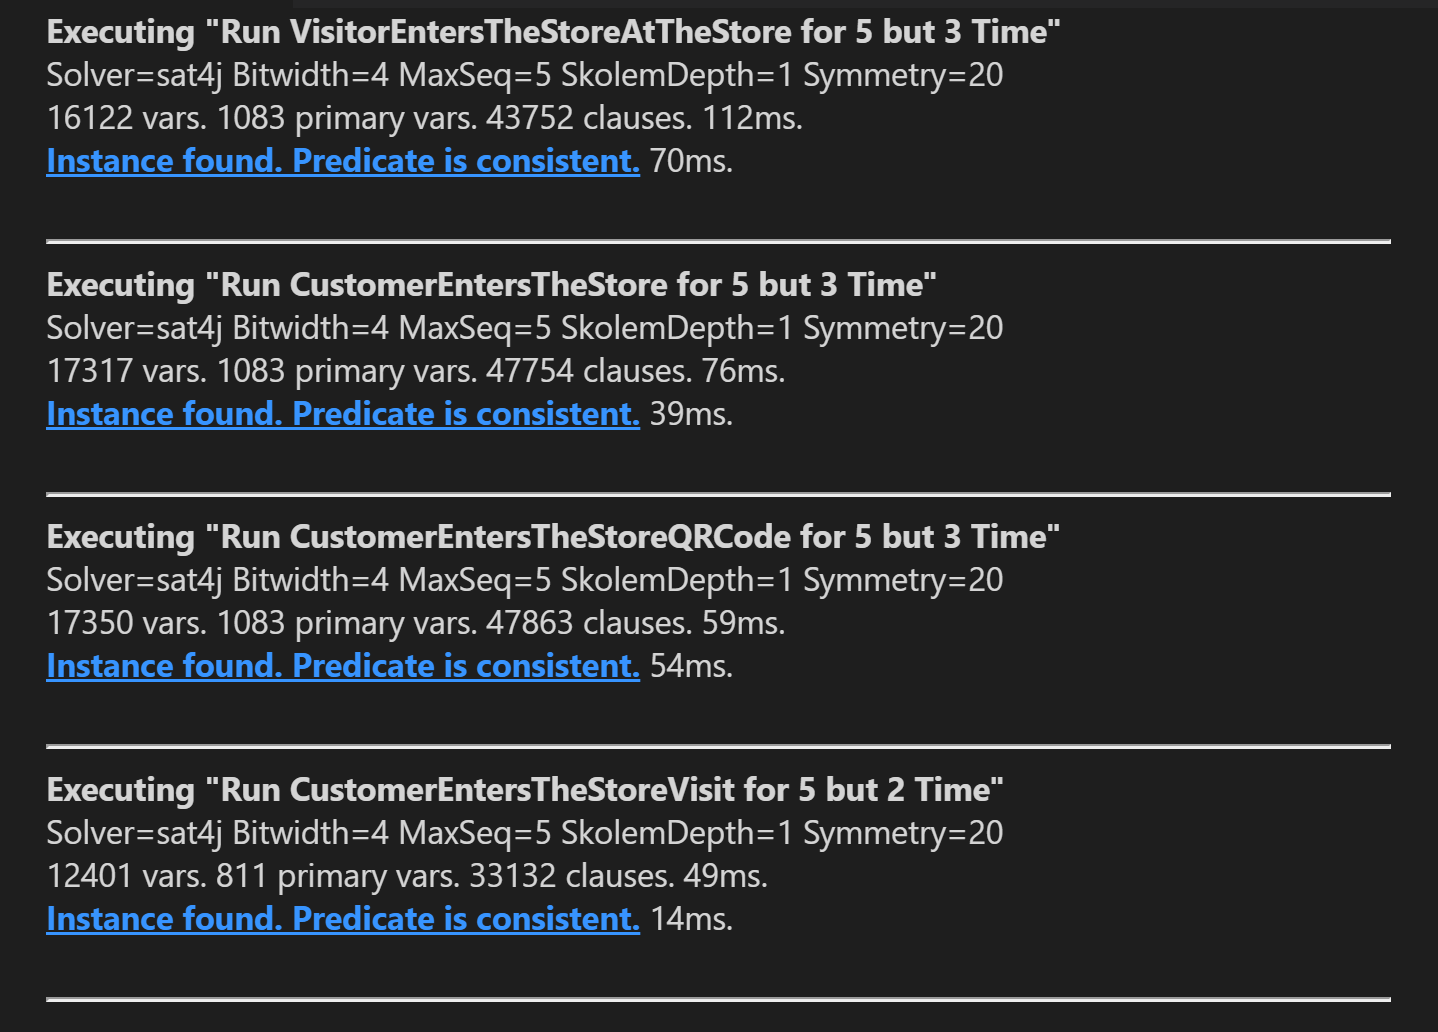
\includegraphics[width=10cm]{proof_of_consistency.png}
    \end{center}

\subsection{Generated world}
Here we include one generated world related to the CustomerEntersTheStoreQRCode pred. The 3 images show the evolution over time of the generated world. We can notice that the Customer is called when the estimatedQueueTime equals the estimatedTravelTime (fig 4.2), that the Entrance is checked through the QRCode and not by an employee and that the realTimeOccupancy increases after the entrance (fig 4.3).
\clearpage    

    \begin{figure}
        \centering
        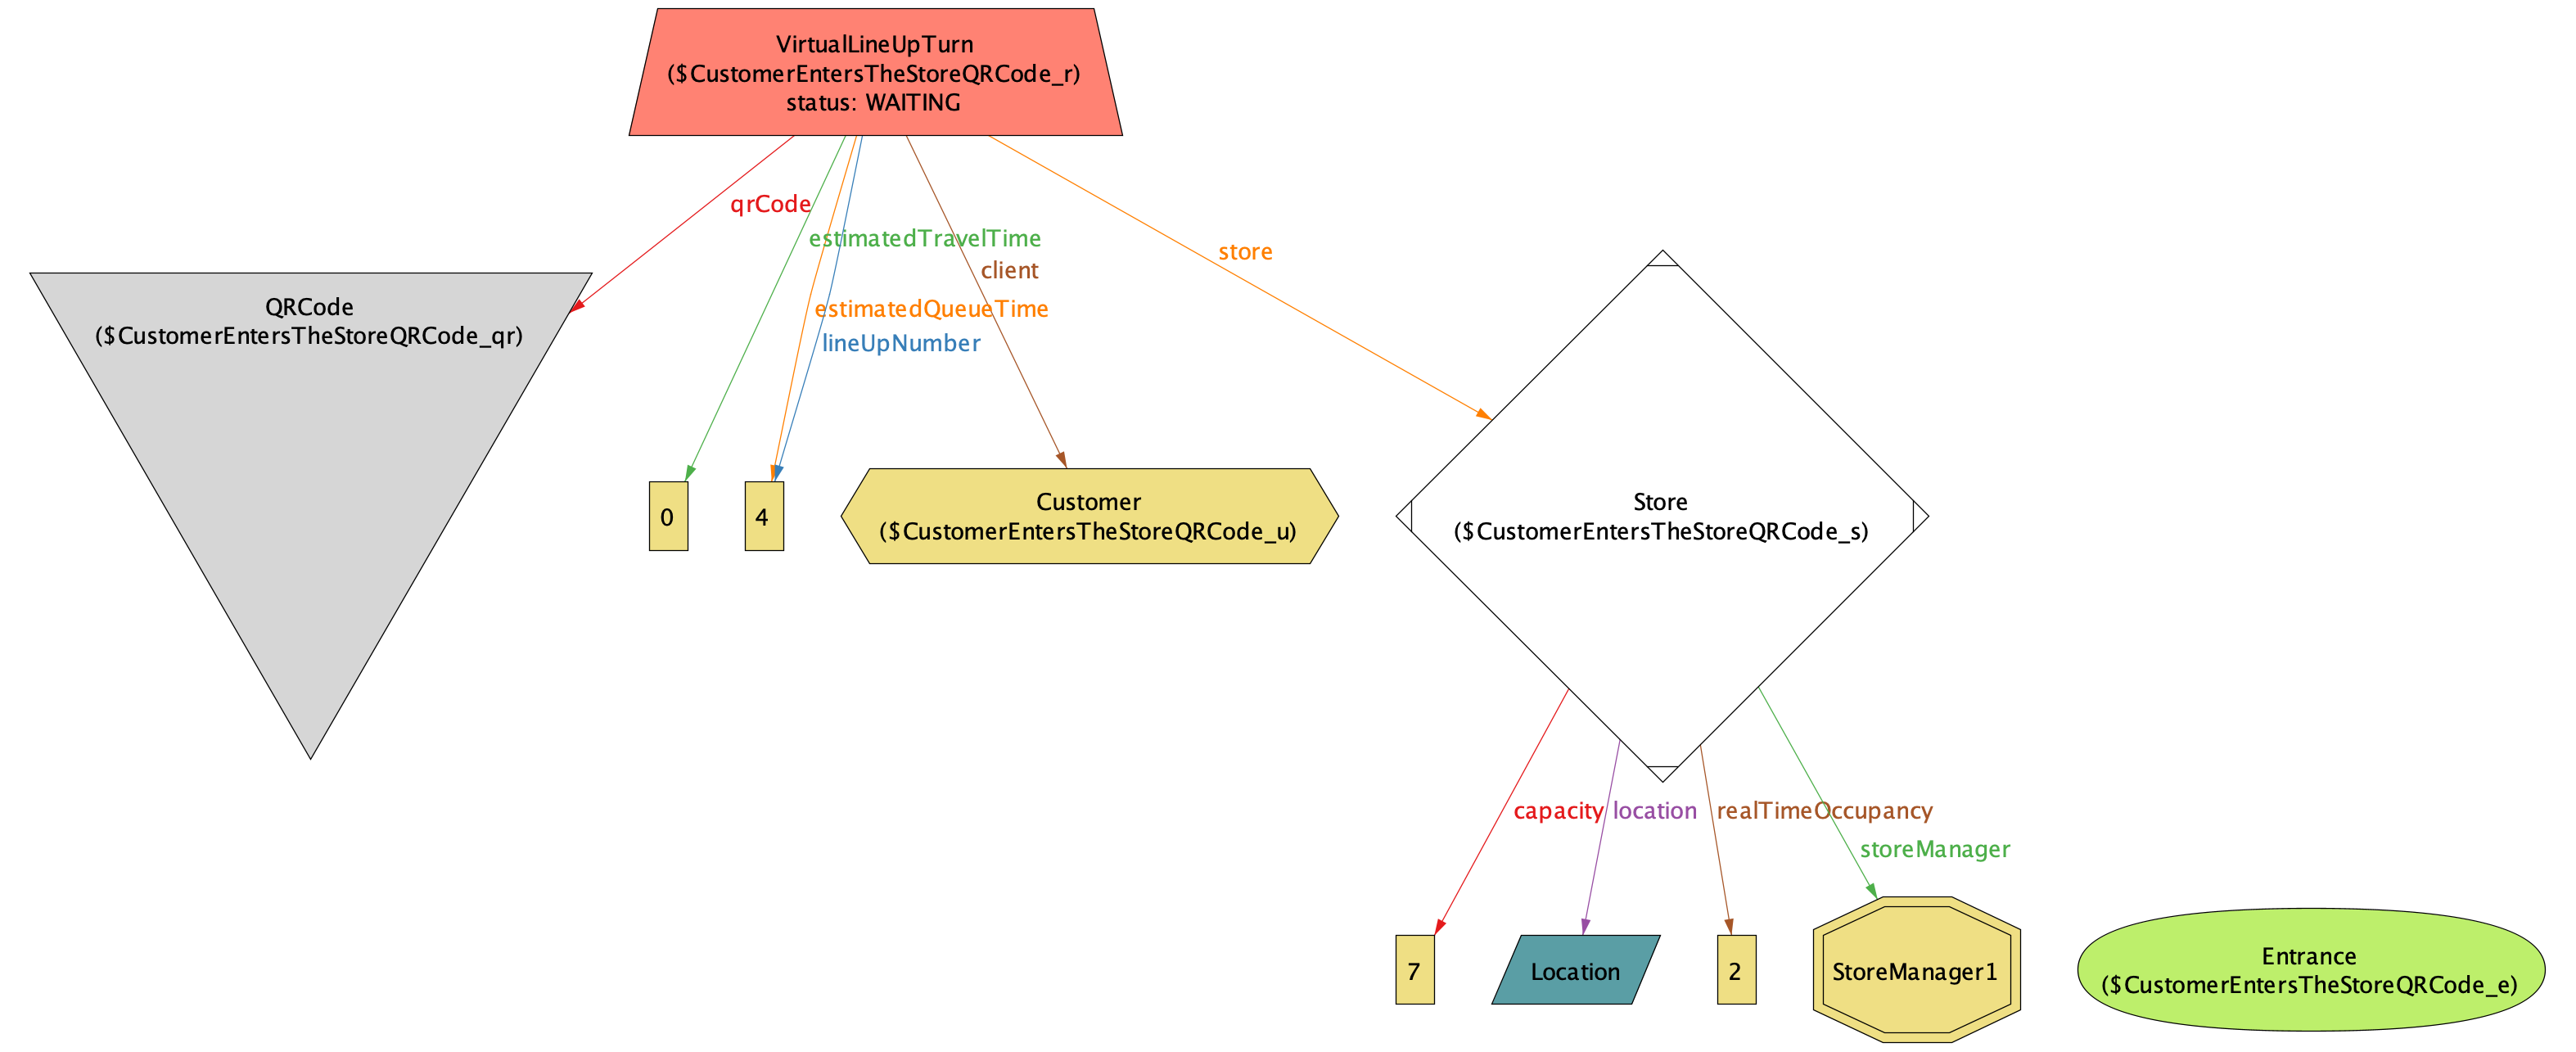
\includegraphics[width=\textwidth]{world1.png}
        \caption{Time0: the Customer is waiting in virtual line}
    \end{figure}
    \begin{figure}
        \centering
        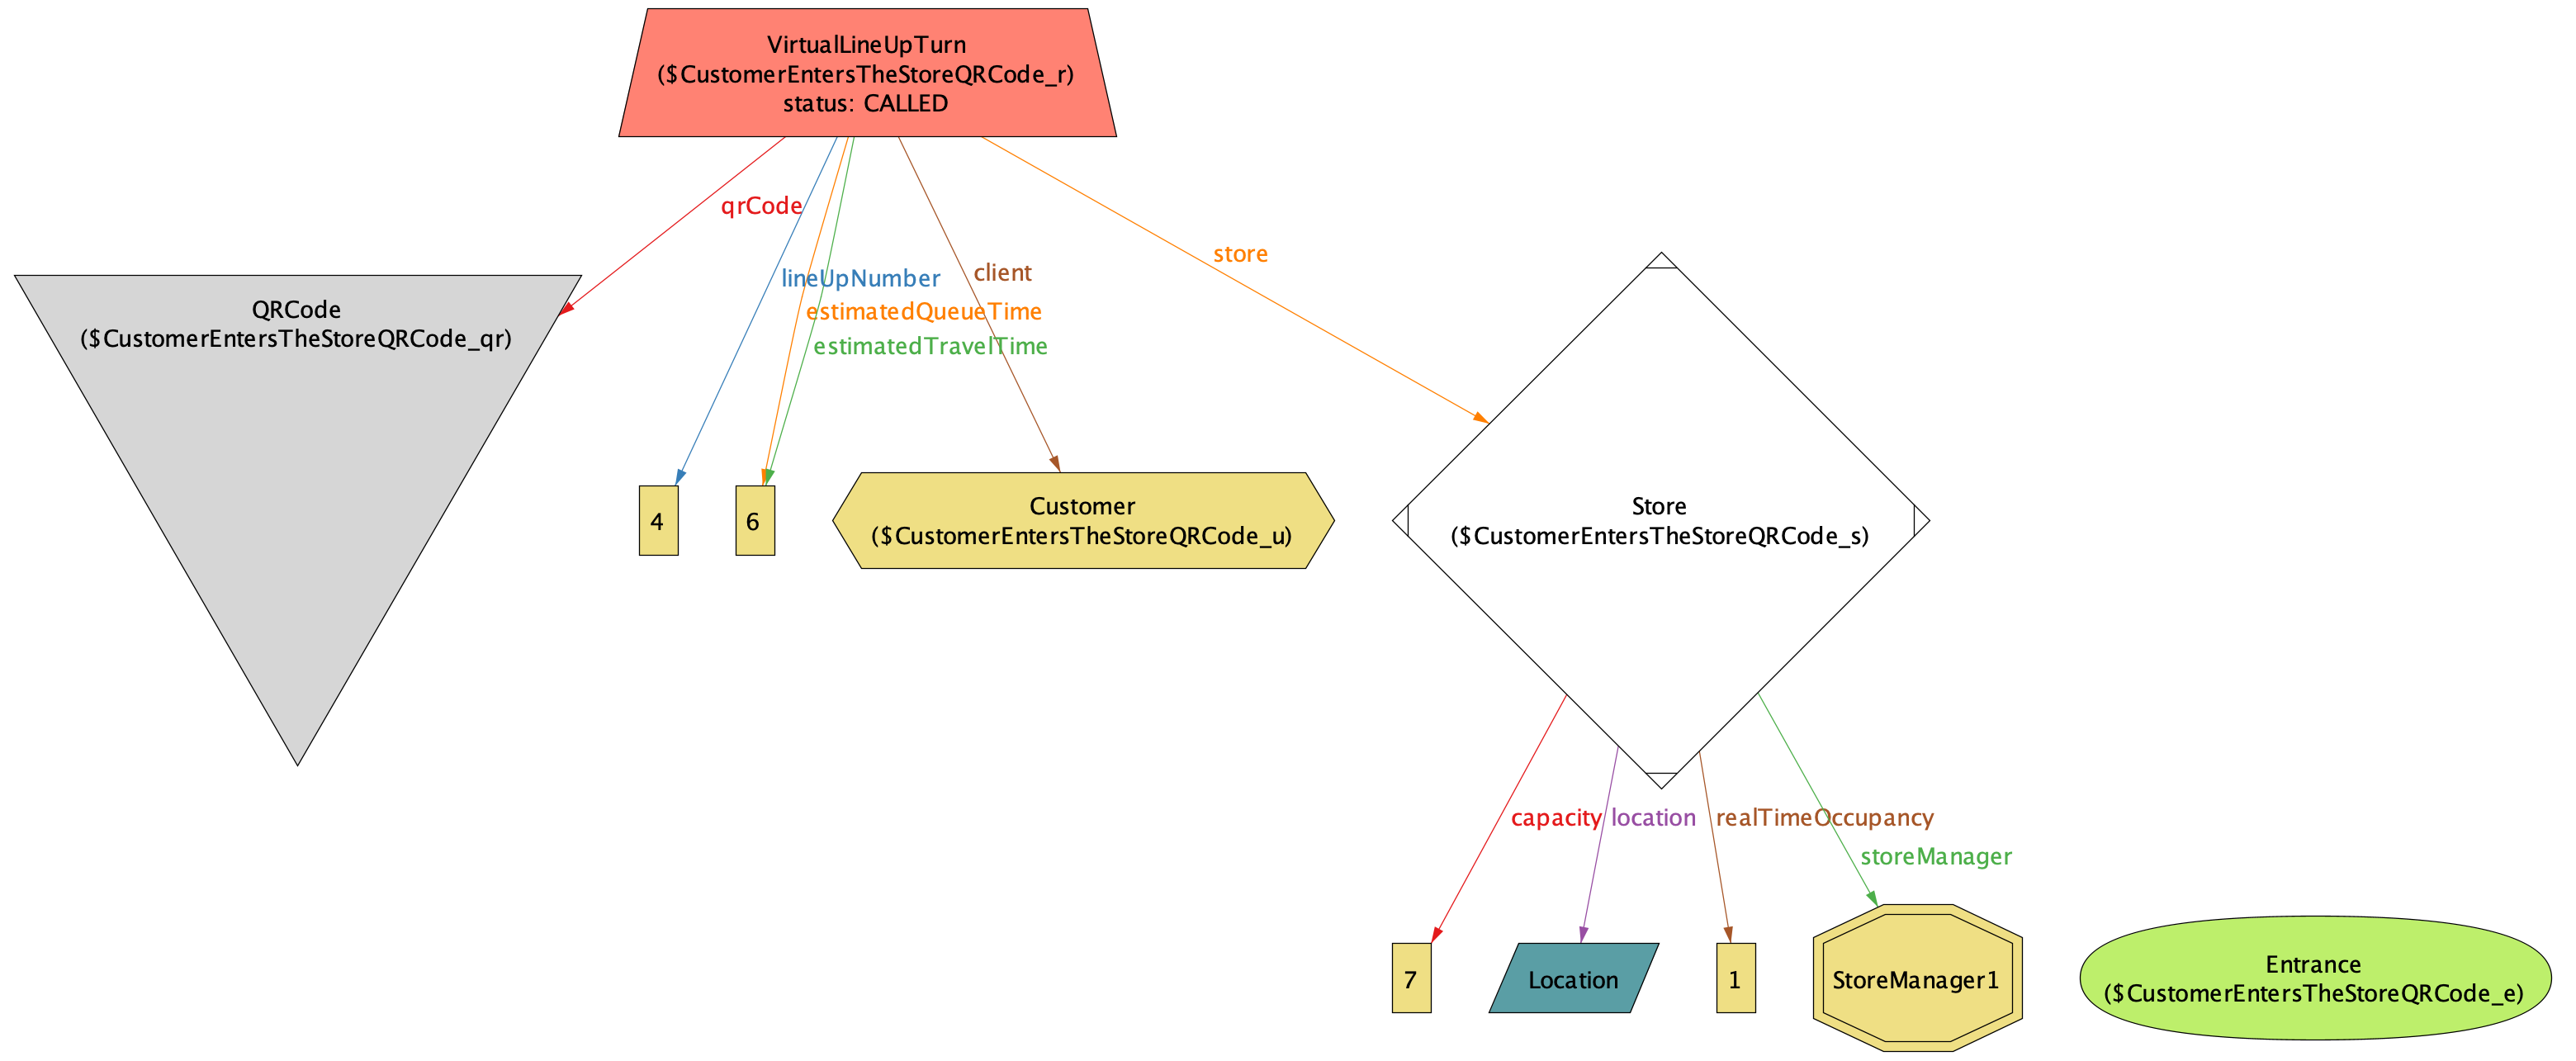
\includegraphics[width=\textwidth]{world2.png}
        \caption{Time1: the Customer is called}
    \end{figure}
    \begin{figure}
        \centering
        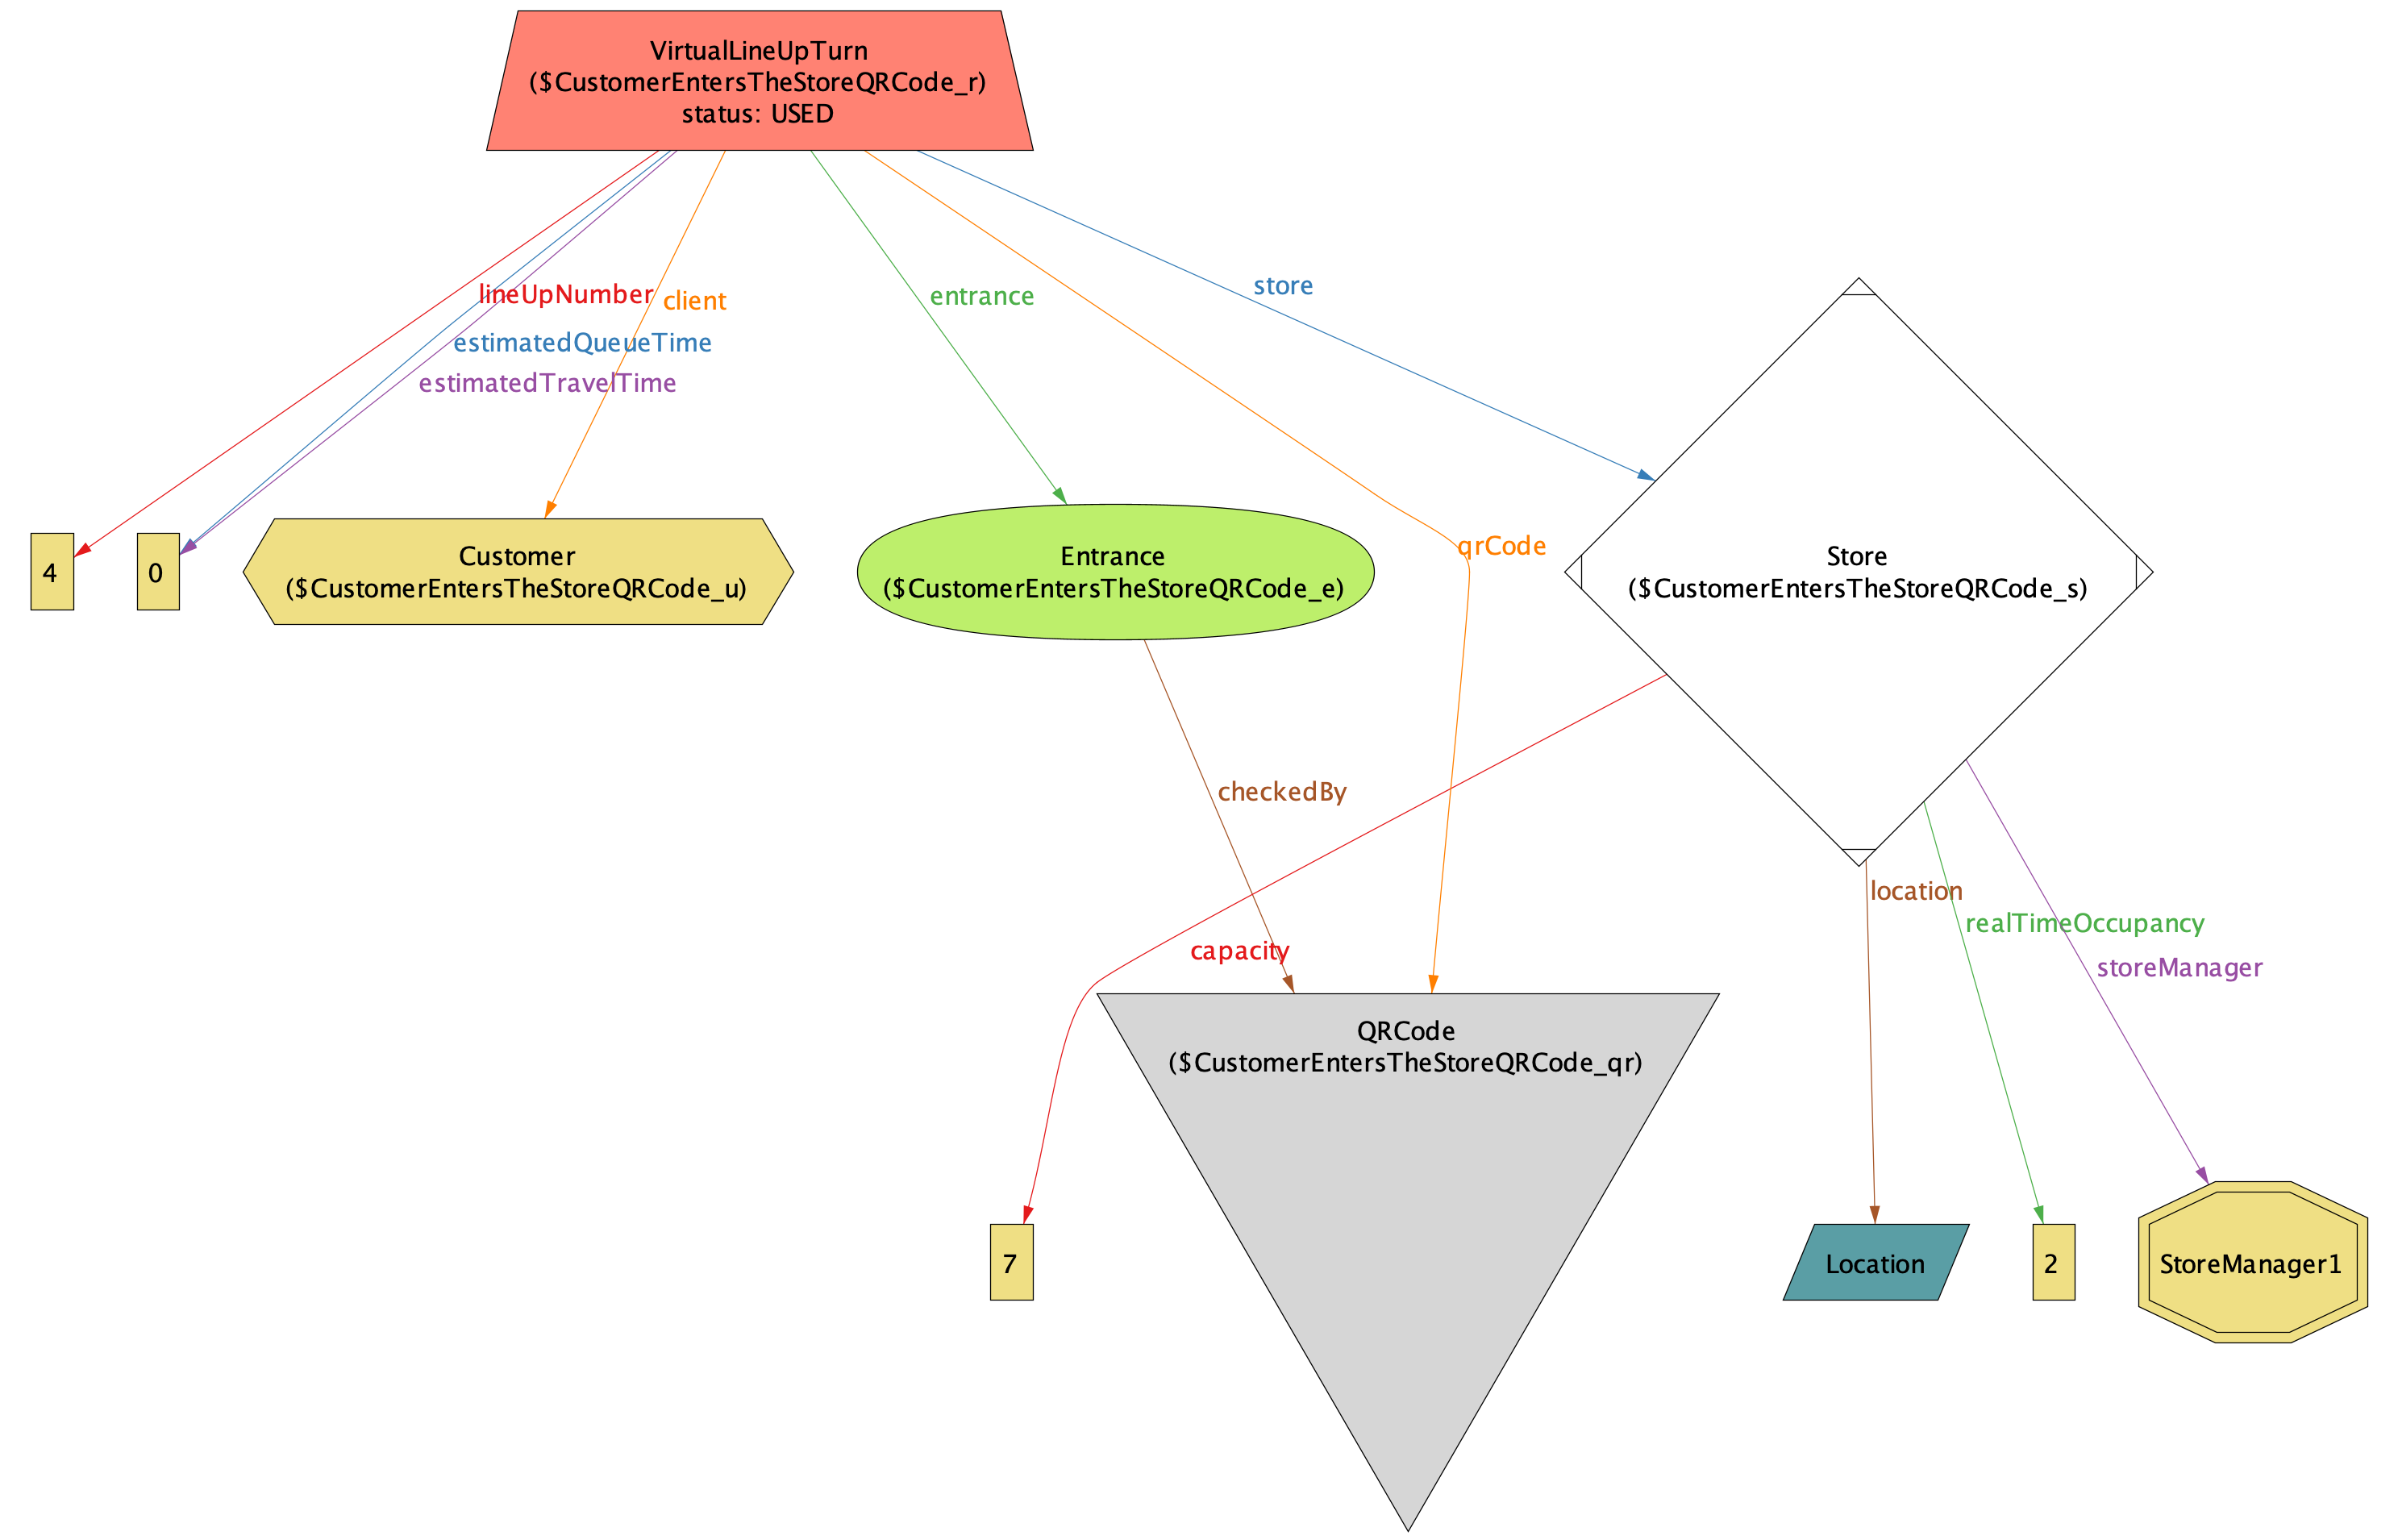
\includegraphics[width=\textwidth]{world3.png}
        \caption{Time2: the Customer enters the Store}
    \end{figure}